\FloatBarrier
\section{Constant False Alarm Rate}
\subsection{Correctness}
Under the assumption of an 8-degrees of freedom chi-squared distribution of sample noise 
power for a given quadruplet of receivers, the CFAR threshold coefficient $\alpha$ is 
calculated numerically for a range of false alarm 
rates. The actual false alarm rate is then measured by running the CFAR algorithm on a noise-only
synthetic dataset. Figure \ref{fig:alpha-cfar-results} illustrates the results.

\begin{figure}[htbp]
    \centering
    \incfig[0.4]{pfa_comparison} 
    \caption[Actual vs desired false alarm rate validating the numerical CFAR threshold.]{The actual 
    false alarm rate closely matches the desired false alarm rate across a range
    of false alarm rates. The numerical solution for $\alpha$ is therefore accurate under the assumption
    of an 8-degrees of freedom chi-squared distribution of sample noise power across a quadruplet of 
    receivers.}
    \label{fig:alpha-cfar-results}
\end{figure}

The results indicate that the numerical solution for $\alpha$ is accurate, with the actual false alarm 
rate closely matching the desired. The successful performance of CFAR with a false alarm rate of 
\(0.001\) is illustrated in Figure \ref{fig:cfar-0.001-waterfall}.

\begin{figure}[htbp]
    \centering
    \incfig[0.8]{cfar-0.001-waterfall}
    \label{fig:cfar-0.001-waterfall}
    \caption[CFAR waterfall at false alarm rate of 0.001.]{CFAR with a desired false alarm rate of \(0.001\) infrequently detects peaks in what is
    predominantly noise, as expected. The figure is a waterfall plot, with chirp on the y-axis and range
    on the x-axis. The brightness of the cell reflects the power of the corresponding chirp's range bin.
    The black space indicates that most cells are masked by CFAR.} 
\end{figure}

\subsection{Computational Performance}
The speed of each of the three CFAR implementations is measured across a range of buffer sizes, from 
one frame of 767 samples, to 4042 frames of 767 samples. This sweep is performed on both the desktop 
and the Xavier. The results are illustrated in Figures \ref{fig:cfar-implementation-performance-Xavier} 
and \ref{fig:cfar-implementation-performance-desktop}.

\begin{figure}[htbp]
    \centering
    \includesvg[width=0.75\linewidth]{CFAR implementation speed on desktop.svg} 
    \caption[CFAR implementation speed vs buffer size on the desktop.]{Computational Performance of three CFAR implementations as a function of buffer size on the
    desktop setup. The CPU implementation with a prefix sum tables is the fastest for small buffer sizes,
    but the GPU implementation is slightly faster for larger buffer sizes. The naive CPU implementation
    is the slowest across all buffer sizes.}
    \label{fig:cfar-implementation-performance-desktop}
\end{figure}

\begin{figure}[htbp]
    \centering
    \includesvg[width=0.75\linewidth]{CFAR implementation speed on Xavier.svg} 
    \caption[CFAR implementation speed vs buffer size on the Xavier.]{Computational Performance of three CFAR implementations as a function of buffer size on the
    Xavier NX setup. The CPU implementation with a prefix sum tables is the fastest for small buffer sizes,
    but the GPU implementation is slightly faster for larger buffer sizes. The naive CPU implementation
    is the slowest across all buffer sizes.}
    \label{fig:cfar-implementation-performance-Xavier}
\end{figure}

The speed is also plotted as a function of the number of CFAR training cells. The results are illustrated 
in Figures \ref{fig:cfar-implementation-performance-Xavier-training-cells} and 
\ref{fig:cfar-implementation-performance-desktop-training-cells}. The desktop results illustrate that both
the GPU and the prefix sum table implementations are not significantly affected by the number of training
cells, while the naive CPU implementation's speed increases linearly with the number of training cells. 
The Xavier results illustrate that while the prefix sum table implementation remains invariant to the 
number of training cells (as we expect), the GPU implementation's speed does increase with the number 
of training cells, due to the fact that each thread has more work to do to calculate the noise statistic. 
Results on the Xavier show that the GPU implementation is faster than either CPU implementation 
for window sizes within the practical range of 10 - 100 training cells.  

\begin{figure}
    \centering
    \includesvg[width=0.8\linewidth]{CFAR implementation speed over window size 10.svg} 
    \caption[CFAR implementation speed vs training cells on the desktop.]{Computational Performance of three CFAR implementations as a function of the number of
    training cells on the Desktop Setup. Buffer size is fixed at 10 quadruplet chirps per frame.}
    \label{fig:cfar-implementation-performance-desktop-training-cells}
\end{figure}

\begin{figure}
    \centering
    \includesvg[width=0.8\linewidth]{CFAR implementation speed over window size 10 Xavier.svg} 
    \caption[CFAR implementation speed vs training cells on the Xavier.]{Computational Performance of three CFAR implementations as a function of the number of
    training cells on the Xavier Setup. Buffer size is fixed at 10 quadruplet chirps per frame.}
    \label{fig:cfar-implementation-performance-Xavier-training-cells}
\end{figure}

Three implementations of CFAR, CA-CFAR, GO-CFAR, and SO-CFAR, were tested on the DS2 dataset with
six different noise intensities: no noise, -20, -10, 0, 10 and 20dB SNR. Figure 
\ref{fig:cfar-recall} illustrates the recall, the number of 
ground truth range bins with a detection within them, and clutter to signal
ratio as a function of noise and CFAR algorithm. Figure \ref{fig:cfar-clutter-to-signal} 
illustrates the clutter to signal ratio of each of the CFAR algorithms as noise increases, 
and Figure \ref{fig:cfar-position-error} illustrates the RMS position error of the true 
positives of each of the CFAR algorithms as noise increases.  

\begin{figure}
    \centering
    \incfig[0.8]{cfar_recall} 
    \caption[CFAR recall vs noise and algorithm.]{Recall of three CFAR algorithms as a 
    function of noise. The figure shows that the recall decreases with increasing noise, 
    and that CA-CFAR features the lowest clutter power for the noisiest regimes.}
    \label{fig:cfar-recall}
\end{figure}

\begin{figure}
    \centering
    \incfig[0.8]{cfar_clutter_to_signal} 
    \caption[CFAR clutter to signal ratio vs noise and algorithm.]{Clutter to signal 
    ratio of three CFAR algorithms as a function of noise. The figure shows that the 
    clutter to signal ratio increases with increasing noise, and that CA-CFAR 
    features the lowest clutter power for the noisiest regimes, while GO-CFAR 
    performs well in the low noise intensities.}
    \label{fig:cfar-clutter-to-signal}
\end{figure}

\begin{figure}
    \centering
    \incfig[0.8]{cfar_position_error} 
    \caption[CFAR position error vs noise and algorithm.]{RMS position error of the 
    true positives of three CFAR algorithms as a function of noise. The figure shows 
    that the position error increases with increasing noise, and that all CFAR 
    algorithms perform with similar accuracy. CA-CFAR features slightly better 
    accuracy in the noisiest regimes }
    \label{fig:cfar-position-error}
\end{figure}

\subsection{Clustering}
The clustering stage is validated on the DS2 dataset with no noise. The ground truths are 
depicted in Figure \ref{fig:angle-3d-plot}. The results are illustrated
in Figure \ref{fig:clustering-results}. The figure shows that the clustering stage successfully
maps contiguous blocks of detected range bins into single detections with continuous
range. 

\begin{figure}
    \centering
    \incfig[0.9]{cluster-experiment}
    \caption[Clustering results on the DS2 dataset with no noise.]{Clustering results on the 
    DS2 dataset with no noise. The figure shows that the clustering stage successfully
maps contiguous blocks of detected range bins into single detections with continuous
range. The y-axis is time and the x-axis is range. The colour is amplitude. The bright 
pink line in the first two subplots corresponds to the green and yellow line in the cluster 
output.}
    \label{fig:clustering-results}
\end{figure}


\subsection{Monopulse Angle Sensing}
\subsection{Correctness}
With the same DS2 dataset from the CFAR evaluation with 0 noise, the monopulse angle sensing 
algorithm is validated by comparing it's azimuth and elevation estimates to the ground truth. 
The results are illustrated in Figures \ref{fig:angle-polar-error} and 
\ref{fig:angle-3d-plot}. Seeing low error suggests that the monopulse angle sensing is 
correctly applying the reverse transformation that the radio wave simulation piece utilised
to convert position to multi-change signal data. 

\begin{figure}
    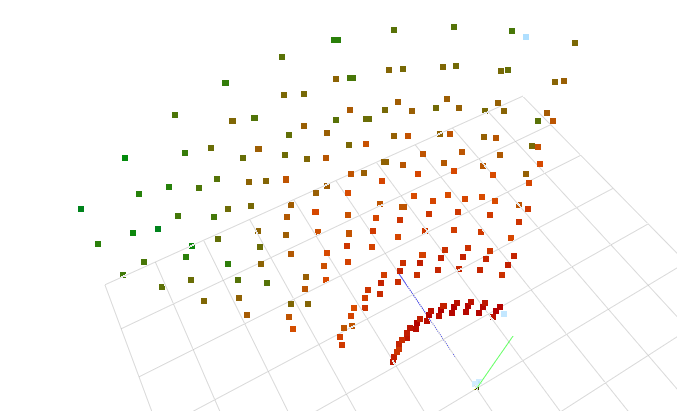
\includegraphics[width=0.8\textwidth]{angle-ground-truth-3d.png}
    \centering
    \caption[Angle experiment Ground Truth 3D plot]{The ground truth measurements of the angle sensing DS2
    dataset plotted in 3D. Points are coloured by signal strength and points are arranged in a 
    polar array.}
    \label{fig:angle-3d-plot}
\end{figure}

\begin{figure}
    \incfig[0.8]{angle_polar_error_scatter_plot}
    \centering
    \caption[Monopulse angle sensing polar error scatter plot.]{Polar error scatter plot
    of the monopulse angle sensing algorithm on the DS2 dataset with 0 noise. The figure 
    shows that the polar error of the angle estimates is generally below 0.3 degrees in 
    az el and rng and the range error is less than 1.5 meters over the tested range. } 
    \label{fig:angle-polar-error}
\end{figure}

Under -10dB SNR, the 3D plot view fills up with clutter and angle sensing accuracy 
quickly degrades. But plotting the amplitude of the detections and accumulating 
detections over 64 chirps per grid position in the dataset, clusters around the 
true target positions can be visually identified, validating the effectiveness of 
monopulse angle sensing in high noise conditions (calculated azimuth and elevation
seem to be unbiased estimators of the true azimuth and elevation). The phenomenon 
is illustrated in Figure \ref{fig:angle-3d-plot-noise}.

\begin{figure}
    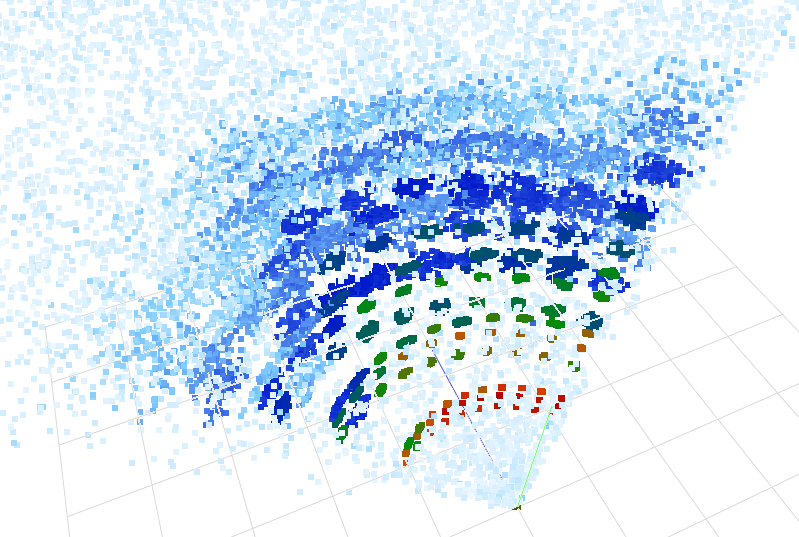
\includegraphics[width=0.7\linewidth]{angle squares light mode noisy.png}
    \caption[Monopulse angle sensing 3D plot with noise.]{3D plot of the monopulse 
    angle sensing algorithm on the DS2 dataset with -10dB SNR at max range. The 
    figure shows the 
    degradation in angle sensing accuracy under high noise conditions as range increases}
    \label{fig:angle-3d-plot-noise}
\end{figure}

To understand the failure modes of monopulse angle sensing for multiple targets, 
a simulation tool was built to validate the monopulse angle sensing algorithm on 
synthetic data. The tool allows the 
user to create multiple targets, and specify the bearing/elevation ratios of each 
target. The simulated data is then 
processed by the preprocessing subsystem, the aggregator, CFAR, and the monopulse 
angle sensing algorithm. The 
resulting angle estimates are visualised live in a 3D plot. A frame of this view is 
illustrated in Figure 
\ref{fig:monopulse-angle-sensing-results}.

\begin{figure}
    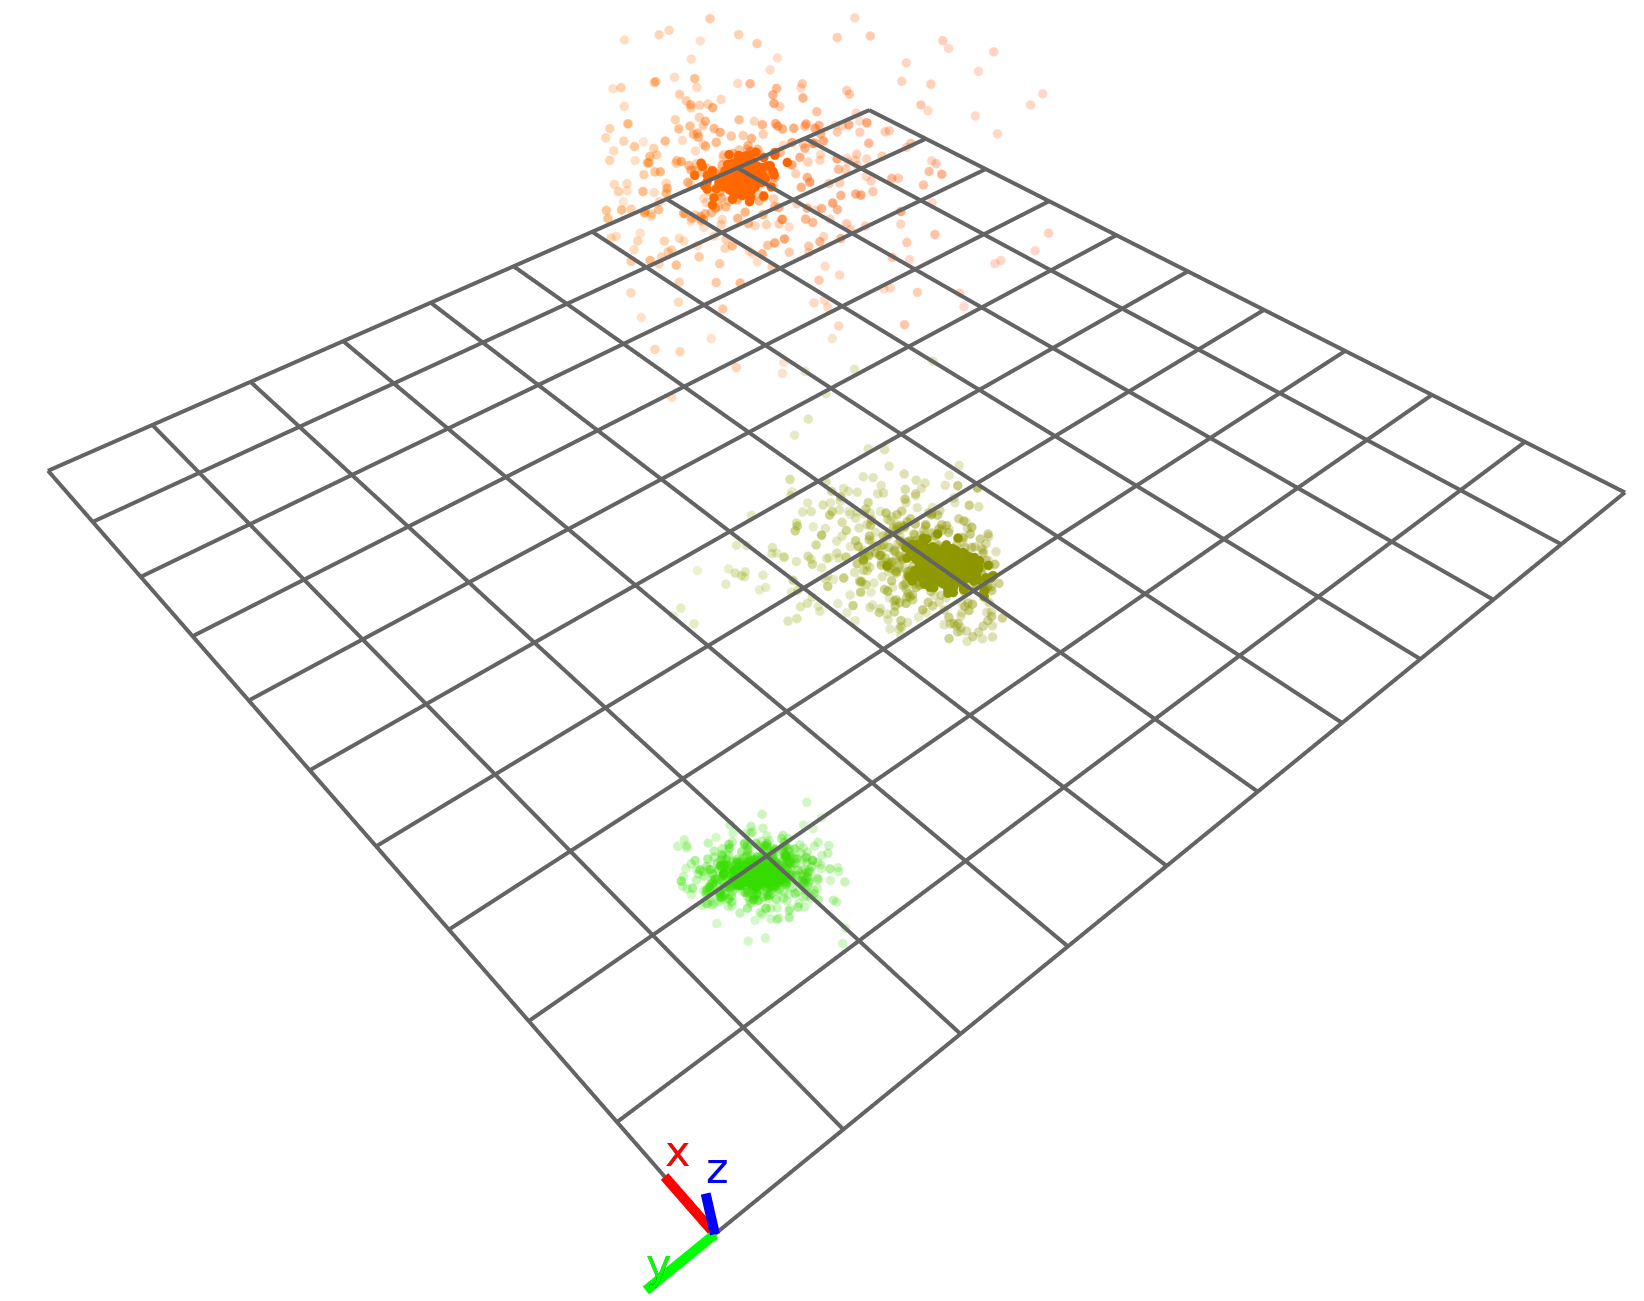
\includegraphics[width=0.8\linewidth]{monopulse_angle_sensing_results.png}
    \caption[Monopulse angle sensing results on synthetic data.]{Results of the monopulse angle sensing algorithm on synthetic data. The colour of the dots indicate
    the range of the detections, with green being close and orange being far away. The opacity of the dots indicate
    the strength of the detections, with more opaque dots being stronger. The plot features the most recently 1000
    detections. The spread of the dots increases with range as expected, and the
    upper and lower bounds of elevation and bearing match the field of view
    defined by the calibration polynomial.}
    \label{fig:monopulse-angle-sensing-results}
\end{figure}

The relative latency cost of the angle and CFAR operations were measured through an ablation study on the detection 
subsystem. The results are illustrated in Figure \ref{fig:tracking-latency-trials} which shows the latency 
of just CFAR, just angle sensing, and both, and Figure \ref{fig:tracking-latency-breakdown}. 

\begin{figure}
    \includesvg[width=0.8\linewidth]{tracking_latency_trials.svg}
    \caption[Detection subsystem latency for CFAR, angle sensing, and both.]{Latency of the subsystem running CFAR, angle sensing, and both on a log scale.
    The latency of the subsystem
    running CFAR is similar to the latency of the subsystem running both, while angle sensing
    is 1.5-5 times faster than either,
    suggesting that CFAR dominates the latency of the subsystem.}
    \label{fig:tracking-latency-trials}
\end{figure}

\begin{figure}
    \includesvg[width=0.8\linewidth]{tracking_latency_breakdown.svg}
    \caption[Detection subsystem latency breakdown from ablation study.]{A breakdown of the latency of the subsystem estimated from the ablation study.
    Most of the latency is split
    between CFAR and the overhead of handling the data, which involves synchronising threads
    and migrating data between the CPU and GPU.}
    \label{fig:tracking-latency-breakdown}
\end{figure}

The angle stage has no parameters to tune other than the coefficients of the calibration
polynomial, which are determined by the beam shape of the receivers. Therefore, the latency 
and correctness analysis is all that can be done. 

\subsection{Tracking}
To validate the tracking stage, 12 scenarios were selected from the DS2 dataset. 
These scenarios involve 1, 2 and 3 targets at no noise, -20, -10, and 0 SNR. Figures 
\ref{fig:tracking-initiation-accuracy} and \ref{fig:tracking-position-accuracy} 
demonstrate the effect of noise and target count on track initiation accuracy, 
position accuracy, and track health.  

%include 4 figures
% track_basic_stats
% track_MOTA_stats
% track_RMS Angle Error
% track_RMS Distance

\begin{figure}
    \incfig[1]{track_basic_stats}
    \caption[Tracking initiation accuracy and track health.]{Tracking accuracy and 
    track health across 12 scenarios with different noise and target count. The figure shows 
    that track-level accuracy, precision, recall, are highest when there is some noise, and 
    only one target. Point level accuracy, precision and recall are also highest in that 
    scenario.}
    \label{fig:tracking-initiation-accuracy}
\end{figure}

\begin{figure}
    \incfig[1]{track_MOTA_stats}
    \caption[Tracking MOTA (Multi-Object Tracking Accuracy) statistics.]{MOTA is highest in the presence of some 
    noise and one target. MOTP (Multi-Object Tracking Precision) strictly increases with noise for all target 
    counts. Mean completeness, mean delay until initiation, fragmentation, and survival 
    ratio are also depicted. }
    \label{fig:tracking-position-accuracy}
\end{figure}

\begin{figure}
    \incfig[0.8]{track_RMS_Angle_Error}
    \caption[Tracking RMS angle error.]{Tracking RMS angle error across 12 scenarios 
    with different noise and target count. The figure shows that RMS angle error 
    degrades with increasing noise and target count.}
    \label{fig:tracking-angle-error}
\end{figure}

\begin{figure}
    \incfig[0.8]{track_RMS_Distance}
    \caption[Tracking RMS distance error.]{Tracking RMS distance error across 12 scenarios 
    with different noise and target count. The figure shows that RMS distance error 
    degrades with increasing noise and target count.}
    \label{fig:tracking-distance-error}
\end{figure}

% Here include basic stats and fancy stats. 
% Talk more about random targets instead of sweep
% Show the ground truth for three targets and some view-tracks.py images. 
% Get everyone to understand how much the tracking stage is doing.